
\section{Introduction}
\label{section:intro}
In this report, we will provide the results of a careful investigation of the performance of the software packages applied to a typical initial value ordinary differential problem encountered in Covid-19 modelling. 

For any mathematical model, the relevance of the solution should be determined by the quality of the model and the accuracy of the parameters that appear in the model. Numerical errors associated with the computational techniques that are used to obtain the solution must always be negligible. Researchers deserve to obtain numerically accurate solutions to the models that they are studying. In this report, we will show that the straightforward use of standard IVODE solvers on typical Covid-19 models can lead to numerical solutions that have large errors, some of the same order of magnitude as the quantities being researched.

In Section $\ref{subsection:research_papers}$, we review how IVODES are used in epidemiology. In Section $\ref{subsection:SEIR_model}$, we define the SEIR models which we will consider throughout this paper, in Section $\ref{subsection:exponential_growth}$, we discuss the problem of stability as it concerns problems with exponential growth, in section $\ref{subsection:fixed_vs_control}$, we explain the difference between fixed step-size and error-controlled solvers and in section $\ref{subsection:effect_of_discontinuity}$, we discuss the effects of discontinuity on these solvers. The IVODE software packages from programming environments that are typically used by researchers are described in Section $\ref{subsection:numerical_software_used}$. We also make a note of a problem with evaluation at output points that leads to inefficiencies in Section $\ref{subsection:solution_output_points_impl}$

In Section $\ref{subsection:naive_time_problem}$, we apply the solvers to the problem with a time dependent discontinuity and show how this results in numerical solutions with relative errors of the same magnitude as the solution we are trying to compute. In Section $\ref{subsection:time_disc_handling}$, we will use some discontinuity handling to solve the time dependent problem. In Section $\ref{subsection:time_tolerance_study}$, we will use a range of tolerances to discuss the effects of tolerance on the accuracy and efficiency of the solvers.

In Section $\ref{subsection:naive_state_problem}$, we apply the solvers to the problem with a state dependent discontinuity and show how none of the solvers were able to obtain accurate solutions. We will explain how even the use of very sharp tolerances does nothing to improve the models in section $\ref{subsection:state_sharp_tol_failed}$ and show that the only proper way to solve this problem is through event detection, which we will describe in Section $\ref{subsection:intro_event_detection}$. We then show the correct solution to the problem in Section $\ref{subsection:state_with_event_detection}$ and perform a tolerance study on this problem in Section $\ref{subsection:state_tolerance_study}$.

In Section $\ref{section:fortran_inaccuracies}$, we will look through the implementation details for some of the solvers to investigate the cause of the inaccuracies. We conclude the report in Section $\ref{section:summary}$ with a summary and potential for future work

\subsection{Epidemiological modelling}
\label{subsection:research_papers}
One common form of epidemiological study is forecasting. Using previously obtained parameters, the researcher develops a mathematical model involving differential equations which is solved using an ODE solver. Often, the solver will be used to integrate over a large time period so that the researcher can examine how the diseases will spread. For such problems, sharp tolerance values would be used and the solver-problem combination is expected to be resilient over large time periods. In Section $\ref{subsection:exponential_growth}$, we discuss why it is unrealistic to model for large time periods if the infection is still growing exponentially but how measures such as social distancing allow us to reduce modelling errors so we can hope to integrate over longer time periods.

The second type of epidemiology study involve parameter estimation. In this kind of study, data points are collected about on the spread of a virus and we try to fit a mathematical model through that data. In so doing, we can estimate the parameters used by looking at which parameters minimise the error in the fit. The parameters estimated, as such, can tell us if implemented control measures are working and may point out what can be done to improve the situation. An example of such a study can be found in Section $\ref{section:ebola_paper}$. Also, parameters so estimated can be used for the first kind of study. Parameter estimation studies often involves using an ODE solver inside a regression or optimisation algorithm and thus the computing time, especially with large problems, can be significant. We will therefore investigate whether or not researchers can coarsen the tolerance.

\subsection{Detailed description of two specific models to be considered in this report.} 
\label{subsection:SEIR_model}
(Reference Christina Christara.)
In this section, we describe the models that we are going to use. They involve typical SEIR models to which we add discontinuities.

The model is as follows:

\begin{equation}
\frac{\textit{d}S}{\textit{dt}} = \mu N - \mu S - \frac{\beta}{N}IS \nonumber
\end{equation}

\begin{equation}
\frac{\textit{d}E}{\textit{dt}} = \frac{\beta}{N}IS - \alpha E - \mu E \nonumber
\end{equation}

\begin{equation}
\frac{\textit{d}I}{\textit{dt}} = \alpha E - \gamma I - \mu I \nonumber
\end{equation}

\begin{equation}
\frac{\textit{d}R}{\textit{dt}} = \gamma I - \mu R \nonumber
\end{equation} 

In this SEIR model, we describe the epidemic over time. S is the number of susceptible individuals, E is the number of exposed individual, I is the number of infected individuals and R is the number of recovered individuals at a point in time. We also use N to represent the population size.
The parameters in this model are as follows: $\alpha$ is such that $\alpha^{-1}$ is the average incubation period, $\beta$ is the transmission rate, $\gamma$ is the recovery rate and $\mu$ is the replenishment rate. In this report, we assume that all these parameters are known as our goal is to investigate the solvers. We will see that we get solutions that are not efficiently computed or that may have significant errors. This issue can have serious consequences as it will fail to show the actual impact of the virus as it corresponds to the actual epidemiology theories behind the mathematical models. These incorrect numerical solutions may trick epidemiologists into giving wrong conclusions and try to change the mathematical models themselves when it is the solvers which are at fault.

The discontinuity we are going to consider involve the parameter $\beta$.
Before measures such as social distancing and others are implemented, $\beta$ has a much higher value than after. In our case, $\beta$ will be 0.9 before the measures and 0.005 after they are implemented. Such abrupt changes in a modelling parameter introduces a discontinuity as we will show in Section $\ref{subsection:effect_of_discontinuity}$. 

In the time dependent discontinuity, we will assume that at some point in time, measures are implemented that will lead to a reduction in the parameter $\beta$. We would like to model the problem through this discontinuity but as we will show, this discontinuity introduces a numerical issue.

In the state dependent discontinuity, we consider the following situation. If the population of exposed people reaches a certain maximum threshold, measures are introduced which decreases the value of $\beta$. This create a discontinuity. Then, when the population of exposed people drops below a certain minimum threshold, the measures are relaxed which increase $\beta$ back, which is another discontinuity. We will try to model this problem through a long time period corresponding to the 'waves' of the pandemic. We note that each time we change the parameter $\beta$, a discontinuity is introduced and thus this problem is far more discontinuous than the previous one, which had only one discontinuity. In so doing, we show that all the solvers will fail.

The other parameters are assumed to always be constant with N at 37,741,000 (the approximate population size of Canada), $\alpha$ at 1/8, $\gamma$ at 0.06 and $\mu$ at 0.01/365.

The initial values are E(0) = 103, I(0) = 1, R(0) = 0 and S(0) = N - E(0) - I(0) - R(0).

This gives us a complete system of initial value ordinary differential equations that is in a form that can be solved by typical software packages.

\subsection{Exponential Growth and the problem of instability}
\label{subsection:exponential_growth}
It turns out that some of the solutions components to the SEIR model exhibit exponential growth over certain time periods. In this section, we discuss exponential growth and its impact on the computation of numerical solution. First of all, we give a quick overview of stability for ODEs. Then we will show that the SEIR model is unstable and how measures such as social distancing can improve the stability. This is important as this essentially means that before measures are implemented, accurate models are for the most part impossible but the addition of the measures such as social distancing can give us hope that our solvers will perform better.

The stability of an ODE is associated with the impact of small changes to the initial values on the solution to the problem. An ODE is unstable if a small change in the initial value results in drastically different solutions, the ODE is said to be stable.

It is straightforward to see that the solution to problems that exhibits exponential growth are unstable. This is the case with Covid-19 modelling. The population of infected people grow exponentially for as long as there are no measures or the number of infected people is small compared to the size of the population. This means that ODE solvers will experience difficulties in obtaining accurate numerical solutions even if we are slightly wrong in our initial estimate of the number of infected people. 

In Figure $\ref{fig:unstability_of_exponential_growth}$, we show exponentially growing solutions corresponding to models with slightly different initial value of E(0). We can see that we get different solutions.

\begin{figure}[h]
	\centering
	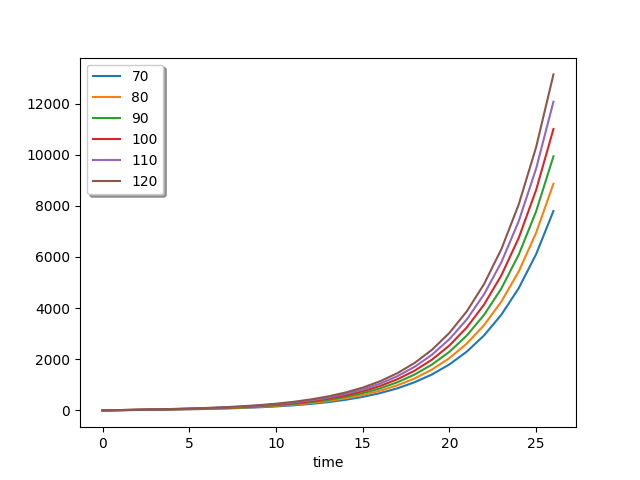
\includegraphics[width=0.7\linewidth]{./figures/unstability_of_exponential_growth}
	\caption{Instability of exponential growth}
	\label{fig:unstability_of_exponential_growth}
\end{figure}

However, when we introduce measures such as social distancing which leads to a smaller $\beta$ value, the problem will exhibit slower exponential growth or can even show exponential decay. A slower exponential growth means that the solution will not be as sensitive to changes to the initial values. Exponential decay is even better as the solutions from different initial values will converge.

Epidemic modelling problems exhibit this type of behaviour. At first, the problem is unstable but as measures are implemented, which leads to exponential decay rather than growth, the problem becomes very stable. We show this in Figure $\ref{fig:regain_stability_after_measures}$ which is the time dependent problem. At first the solutions diverge during exponential growth, but the addition of measures such as social distancing introduces exponential decay which make them converge. Thus the measures not only save lives but also they improve the accuracy of our solutions as we are less reliant on having accurate initial values.

\begin{figure}[h]
	\centering
	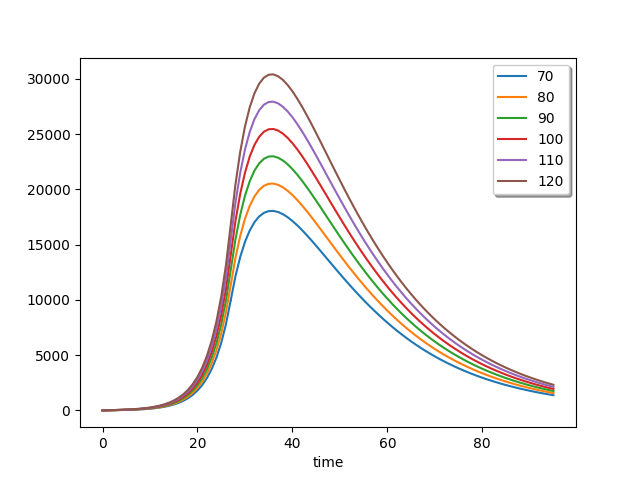
\includegraphics[width=0.7\linewidth]{./figures/regain_stability_after_measures}
	\caption{Gain in stability as measures are implemented}
	\label{fig:regain_stability_after_measures}
\end{figure}

\subsection{Brief overview of numerical software to be employed in the numerical solution of this model}
\subsubsection{Fixed Step Size and Error Control Solvers}
\label{subsection:fixed_vs_control}
We begin our discussion on the software used by giving a brief overview of what is the tolerance and the difference between fixed step size and error control solvers.

The tolerance is a measure of how accurate we want the solution of the solvers to be. Generally, an absolute tolerance of $10^{i}$ means that we want the error estimate to be within $10^{i}$ whereas a relative tolerance of $10^{i}$ means that we want the ratio of the error estimate and the computed solution to be within $10^{i}$. This is not always the case as some solvers will make a blended use of the provided absolute and relative tolerance. This blend is what is going to be compared against error estimate which generally results in more accurate or more efficient solutions

A solver is said to have a fixed step size if it does not have error checking. The solver will have an initial step-size and this step-size is used throughout the whole integration. It will jump from one point to another point in a 'step' and will not check if the step it took was accurate or not. Thus, the distance between the points, i.e the step size, is constant throughout the computation. The only metric that a sharper tolerance will change is the initial step size.

An error controlled solver starts with an initial step size but as it takes a step, it will compute an error estimate and based on the tolerance will recompute the step-size if the error estimate is significant. It will retake the step with a new smaller step size and will repeat the process until the error estimate satisfies the given tolerance. Only then will it move to the next point. Thus it constantly reduces the step-size to step through the problem. This allows it to make sure that the given tolerance is truly satisfied over the whole problem interval.

Error control is not simple to implement. This is where we need to caution against the use of non-standard ODE solvers or other fixed step-size solvers. Also, some researchers, who have an understanding of ODEs may be tempted to write their own solvers. These researchers often program a non-error control method like a simple Euler or a Runge-Kutta method. We will show, using provided fixed step-size solvers in R, how these solvers simply cannot solve a Covid-19 model. Without error control, these solvers cannot handle the discontinuity and stability issues and give very erroneous solutions, often without even a warning that these solutions should not be trusted.

\subsubsection{The packages}
\label{subsection:numerical_software_used}
\subparagraph{R packages}
Scientists who solve ODE models in R commonly use the deSolve package and the $ode()$ function within it.
$ode()$ provides several numerical methods to solve a problem but we have investigated: 'lsoda', 'daspk', 'euler', 'rk4', 'ode45', 'radau', 'bdf' and 'adams'. We note that these are not all the methods provided by the $ode()$ function in R but that the other methods are similar to the ones we are investigating and were thus omitted. The default method is 'lsoda' and the default tolerances are $10^{-6}$ for both the absolute and relative tolerance. We also note that we did not consider the other integrators in the deSolve package like $rkMethod()$, which just present other Runge-Kutta methods, and the other ones which are in-fact called by the $ode()$ function itself.

The error controlled solvers are:
\begin{itemize}
\item Using 'lsoda' calls the Fortran LSODA routine from ODEPACK. It can automatically detect stiffness and choose between a stiff and a non-stiff solver and has error control.
\item Using 'daspk' calls the Fortran DAE solver of the same name. This solver has error control.
\item Using 'ode45' calls an implementation of Dormand-Prince (4)5 (DOPRI5). This solver has error control as it is a Runge-Kutta pair.
\item Using 'radau' calls the Fortran solver RADAU5 which implements the 3-stage RADAU IIA method. This also has error control.
\item Using 'bdf' calls the stiff solver inside the Fortran LSODE package which is based on a family of BDF (Backward Differentiation) methods. It has error control.
\item Using 'adams' calls the non-stiff solver inside the Fortran LSODE package which is based on a family of Adam's methods. It is thus error-controlled. 
\end{itemize}

The fixed step-size solvers are:
\begin{itemize}
\item 'euler' which uses the classical Euler method. It is a fixed step-size solver. It is an implementation in C.
\item 'rk4' which uses the classical Runge-Kutta method of order 4 and thus is a fixed step-size solver.It is an implementation in C. 
\end{itemize}
We will use these methods to demonstrate what happens when researchers program their own non-error controlled solvers as they usually will program similar versions of a classical Euler or a classical Runge-Kutta.

We also make note that R uses the old method to find the values of the solution at output points. This present efficiency issues as we will discuss in Section $\ref{subsection:solution_output_points_impl}$. 

\subparagraph{Python packages}
In Python, researchers use the scipy.integrate package and will normally use the $solve\_ivp()$ function due to its newer interface. It lets the user apply the following methods: 'RK45', 'RK23', 'Radau', 'BDF', 'LSODA' and 'DOP853'. In this report, we will investigate all of these methods. The default solver in $solve\_ivp()$ is 'RK45' and the default tolerance is $10^{-3}$ for the relative tolerance and $10^{-6}$ for the absolute tolerance. 

\begin{itemize}
\item Using 'RK23' uses an explicit Runge-Kutta pair of order 3(2). This uses the Bogacki-Shampine pair of formulas and has error control. It is a Python implementation.
\item Using 'RK45' uses an explicit Runge-Kutta pair of order 5(4). This uses the Dormand-Prince pair of formulas and has error control. It is a Python implementation.
\item Using 'DOP853' uses an explicit Runge-Kutta pair of order 8. The method is error controlled. It is a Python implementation.
\item Using 'Radau' uses an implicit Runge-Kutta method of Radau IIA family of order 5.  The error is controlled with a third-order accurate embedded formula. It is a Python implementation.
\item Using 'BDF' uses a method based on backward-differentiation formulas. This is a variable order method with the order varying automatically from 1 to 5. It is a Python implementation.
\item Using 'LSODA' calls the Fortran ODEPACK for LSODA. This switches between an Adams (nonstiff) and a BDF (stiff) method as it detects stiffness. This is implemented in Fortran.
\end{itemize}

We note that all solvers in $solve\_ivp()$ has error control and that only 'LSODA' is using the famous Fortran package itself, the others are a Python implementation and thus might be slow.

\subparagraph{Scilab packages}
In Scilab, researchers solve differential equations with the built-in $ode()$ function which has the following methods: 'lsoda', 'adams', 'stiff', 'rk', 'rkf'. The default integrator is 'LSODA' which is called by not specifying any methods as the first argument.
Default values for the tolerances are respectively $10^{-5}$ for the relative tolerance and $10^{-7}$ for the absolute tolerance for all solvers used except "rkf" for which the relative tolerance is $10^{-3}$ and the absolute tolerance is $10^{-4}$.
This means that "rkf" has a coarser default tolerance. We will see that this is relevant for this investigation.

\begin{itemize}
\item the default is 'lsoda' which will call the Fortran LSODA code from ODEPACK. This switches between an Adams (nonstiff) and a BDF (stiff) method as it detects stiffness. It has error control.
\item Using 'stiff' calls the stiff solver inside Fortran's LSODE package which is based on a family of BDF (Backward Differentiation) methods. It has error control.
\item Using 'adams' calls the non-stiff solver inside Fortran's LSODE package which is based on a family of Adam's methods. It is error-controlled.
\item Using 'rk' calls an adaptive Runge-Kutta method of order 4. It has error control and uses Richardson extrapolation for the error estimation. It is implemented in Fortran in a file called 'rkqc.f'.
\item Using 'rkf' calls the Shampine and Watts program based on Fehlberg's Runge-Kutta pair of order 4 and 5 (RKF45) pair. It is error-controlled and calls the Fortran rkf45.f.
\item daskr????
\end{itemize}

\subparagraph{How the packages relate}
We tried to find the connections across the programming environment where the solvers appear to be using the same source codes.
Here is what we found:

R's, Python's and Scilab's 'lsoda' are all wrappers around the Fortran LSODA code inside ODEPACK.

R's 'bdf' is equivalent to Scilab's 'stiff' in that they use LSODE's code inside ODEPACK but Python's 'BDF' is a different implementation in Python itself.

R's 'adams' and Scilab's 'adams' are similar in that they both use LSODE's code inside ODEPACK.

R's and Python Runge Kutta 4(5) pairs are both implementations of dopri5 but they have different source code as Python implements its own. Scilab's 'rkf' is not the same pairs as it is using the Shampine and Watts Fehlberg's Runge-Kutta pair not the Dormand-Prince pairs.

Scilab's 'rk' which is of order 4 and R's 'rk4' are not the same solvers. Scilab's 'rk' is adaptive (error-controlled with Richardson extrapolation) whereas R's 'rk4' is a fixed step-size method.

R's 'Radau' and Python's 'Radau' have different source code as Python implements its own 'Radau' code while R seems to be calling the Fortran code.

\subsection{Observation on implementation of solution at output points}
\label{subsection:solution_output_points_impl}
In this section we talk about a problem that we encountered by some ODE solvers in R and Scilab when it comes to plotting. In an ideal scenario, the user's desired output points would not interfere with the efficiency of the solvers. However, in these two platforms, an old method for outputting is used which makes asking for a lot of output points very inefficient.

Normally, an ODE solver will work as such: it will have a default initial step-size, will take a step and will adjust the step-size based on the error at the given step and will then use this new step-size to take the next step. This process is repeated until the solver reaches the end of the interval. However, often the users of an ODE solver will require the output at specific points and these points may lie in the middle of a step. The new method to get these output points is to perform an interpolation at the given step and to return the value of that interpolant at the required point.

In R and Scilab, this new method is not used in all the solvers. Instead, R and Scilab will use the vector of output points to dictate the step-size. These solvers will thus use an initial step size or the difference between the start point and the next point as the initial step-size and step to this next point. The solver will then repeat the process between each consecutive pair of points. Thus the space between points will limit the maximum step-size that can be taken and will lead to additional function evaluations because the solver need to pause at each output point. This will lead to a considerable drop in efficiency as we will show, for instance in Tables $\ref{tab:tolerance_time_discontinuity_rk45_R}$ and $\ref{tab:tolerance_time_discontinuity_rk45_further_R}$. These table shows that a problem that can be solved with 150 function evaluation will be solved with 500 function evaluations. This increase in the number of function evaluation will correspond to increases in CPU-time when the ODE function is complex.   

This old method of implementing specific points outputs also means that the accuracy of the solver depends on the space between the desired output points. Both in an error-control and a fixed step-size solver, if the solver needs to pause between each output point the step-size in this interval has a maximum of the difference between the two points. Thus, we get the bizarre behaviour that the accuracy is increased by putting the points closer together and the accuracy is decreased by putting them further apart. We will point out these inconsistencies as they become relevant. We also note that spacing the points closer together is not a precise way to control the accuracy as no researcher will know beforehand how close the points should be.

\begin{figure}[h]
	\centering
	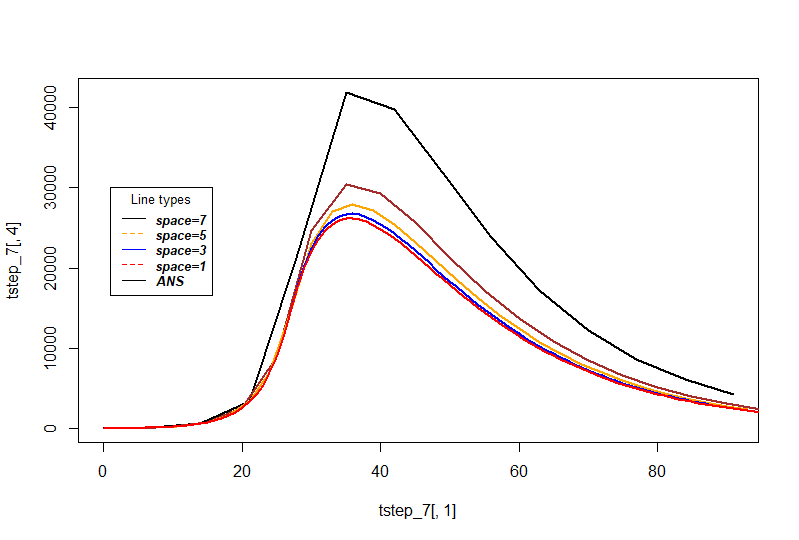
\includegraphics[width=0.7\linewidth]{./figures/R_ode45_spacing_experiment}
	\caption{R 'ode45' spacing between points experiment}
	\label{fig:ode45_spacing_experiment}
\end{figure}

Figure $\ref{fig:ode45_spacing_experiment}$ shows an experiment where we solve an ODE problem using R's 'ode45', which is an implementation of DOPRI5 which has error control but is not using interpolation, to show that it is doing more function evaluation than needed. We set both the absolute and relative tolerance to 0.1 and thus expect poor accuracy but very high performance. However the space between the points is still a limiting factor for the step-size and the solution is somewhat accurate although very inefficient. We recorded the number of function evaluations in Table $\ref{tab:ode45_spacing_experiment}$ and will show that R is using a lot more function evaluations than needed to satisfy such coarse tolerances.

\begin{table}[h]
\caption {R DOPRI5 spacing experiment} \label{tab:ode45_spacing_experiment} 
\begin{center}
\begin{tabular}{ c c }
spacing & nfev \\ 
1 & 572 \\
3 & 188 \\
5 & 116 \\
7 & 80  \\
\end{tabular}
\end{center}
\end{table}

From Figure $\ref{fig:ode45_spacing_experiment}$ and Table $\ref{tab:ode45_spacing_experiment}$, we note that we did not ask the solver for an accurate solution and that it is giving us an excessively accurate solution (too close to the plot of the ANS). This excess accuracy comes at a price of around 500 more function evaluations which is a problem, for instance if the user is running a parameter-estimation-like experiment. Accuracy should ideally be completely determined by the tolerance but using this old method of outputting goes against that. This results in the solvers not being allowed to take as big a step as it can. 

We advise users to use an interpolation software whenever readily available like Python's $dense\_output$ mode in $solve\_ivp$ so that the solvers can run as efficiently as possible. When faster CPU times are required, the researcher can look to see if their chosen solver is using interpolation or if it is making unnecessary stops. If their chosen solver is using the old method, we advise using a different solver whenever possible or running their solvers appropriately spaced out for a set of points and running an explicit interpolation on its output to calculate a smooth curve.

\subsection{Discontinuities and their effects on solvers}
\label{subsection:effect_of_discontinuity}
The main purpose of this paper is to discuss discontinuities and how these affect our models. In this section, we will show what happens when a solver meets discontinuities and how these lead to erroneous solutions.

We need to understand that all the solvers use Mathematical theories based on Taylor Series, one of the core assumption of which is that the functions and all of their relevant derivatives are continuous. If a function is discontinuous, these theories no longer hold and the solvers are no longer guaranteed to converge to the actual solution as the step-size is tend to 0.

We will see that discontinuities will have huge impacts on the efficiency of the solvers, that some solvers, even with error control, will require extremely sharp tolerance to step over them and that fixed step solvers simply cannot solve these problems as they do not reduce the step size accordingly. 

It is important to note that the step that first meets a discontinuity will almost always fail. This is because for the code to step over a discontinuity, the step size need to be much smaller than the one used over a continuous subinterval. The codes will thus have retake the step with a smaller step size and as long as the error estimate is not small enough, it will need to continue retaking the step. This leads to high numbers of function evaluations near the discontinuity which when we have a complex problem will lead to longer CPU times. 

\begin{figure}[h]
	\centering
	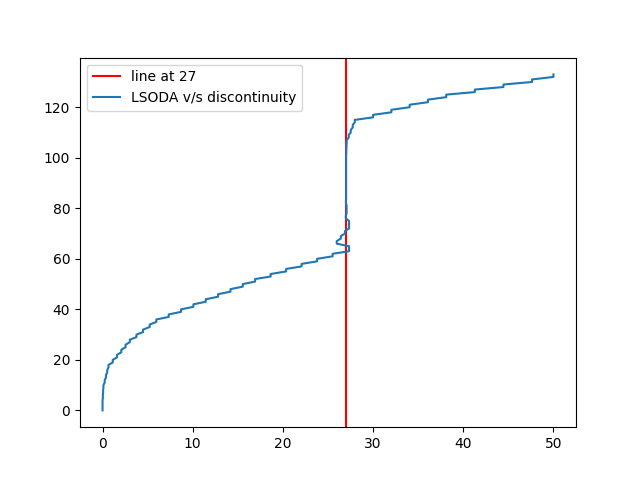
\includegraphics[width=0.7\linewidth]{./figures/lsoda_vs_discontinuity}
	\caption{LSODA against a discontinuity}
	\label{fig:lsoda_vs_discontinuity}
\end{figure}

\begin{figure}[h]
	\centering
	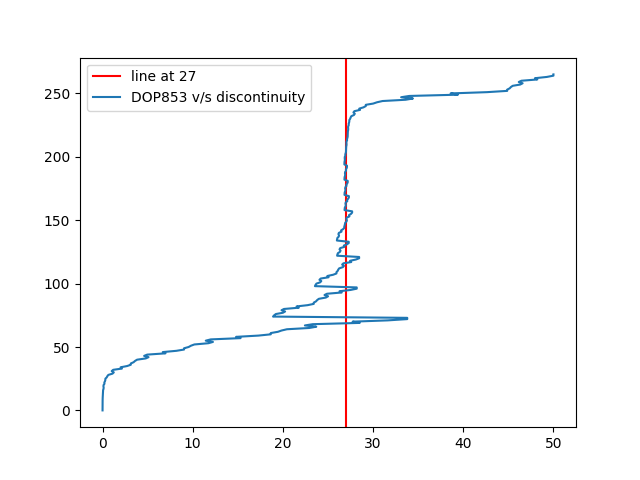
\includegraphics[width=0.7\linewidth]{./figures/dop853_vs_discontinuity}
	\caption{DOP853 against a discontinuity}
	\label{fig:dop853_vs_discontinuity}
\end{figure}

In Figures $\ref{fig:lsoda_vs_discontinuity}$ and $\ref{fig:dop853_vs_discontinuity}$, we run 'LSODA' and 'DOP853' on a discontinuous problem where the discontinuity is at time 27 and plot the time at which the $i^{th}$ function evaluation occurs. We thus show the spike in the number of function evaluations at the discontinuity as the solvers repeatedly retake that step with smaller and smaller step-sizes.

Following this discussion, we also recommend epidemiologists to carry out a manual discontinuity detection experiment to see if their model has any discontinuity. This trivial experiment is done by collecting at what time the solver made the $i^{th}$ call to the solver. The pseudo-code of which is as shown below:

\begin{minipage}{\linewidth}
\begin{lstlisting}[language=Python]
times = []
function_calls = []
count = 0

function model(t, y)
    global times, function_calls, count
    times.append(t)
    function_calls.append(count)
    count += 1	

    // code to find the derivatives
		
    return <derivatives>

plot(times, function_calls)
\end{lstlisting}
\end{minipage}

In the experiment outlined in this pseudo-code, we plot the time against the cumulative count of the function calls. An almost straight vertical line on this graph will indicate that the function was called repeatedly at a specific time and thus that the solver repeatedly changed the step-size in this region to step over a discontinuity. Thus the epidemiologist can detect a discontinuity and can perform further tests. In the remainder of this report, we will outline the ways to accurately and efficiently solve problems with such discontinuities.

VI ============================
ADD A SECTION ON DISCONTINUITY DETECTION ALGORITHM. OR REFERENCES.
A good advice that I will add in my conclusion is to always use a discontinuity detection algorithm if there is if-statements in the ODE function or the epidemiologist suspects a discontinuity.
========================== VI
